\section{Verification of annotation consistency}

\subsection{Check the \emph{PostOffice} project}
Right-click on the \emph{PostOffice} project in the \emph{project explorer} and run the command \emph{Convert SW project to SMV}.
After that, some status information gets printed in the \emph{console view} and a new file with the \emph{.swproj.nusmv} extension
appears in the \emph{project explorer} right next to the \emph{reprotool} project file. You can open the file by double-clicking it
and view it in our \emph{NuSmvLang} editor. The contents of the file will make more sense to you after you read the programming
documentation.

Now, right-click the *.nusmv file and run the \emph{Run NuSMV verification} command. After that, if your \emph{PostOffice} project is
the same as ours, you should notice in the \emph{project explorer} that a file with the extension \emph{.swproj.cexmp} has been
generated. This file tells us that we have some verification failuers in our project. Now view the counter-example file. This situation
is depicted in the next figure.

\begin{figure}[ht]
  \centering
  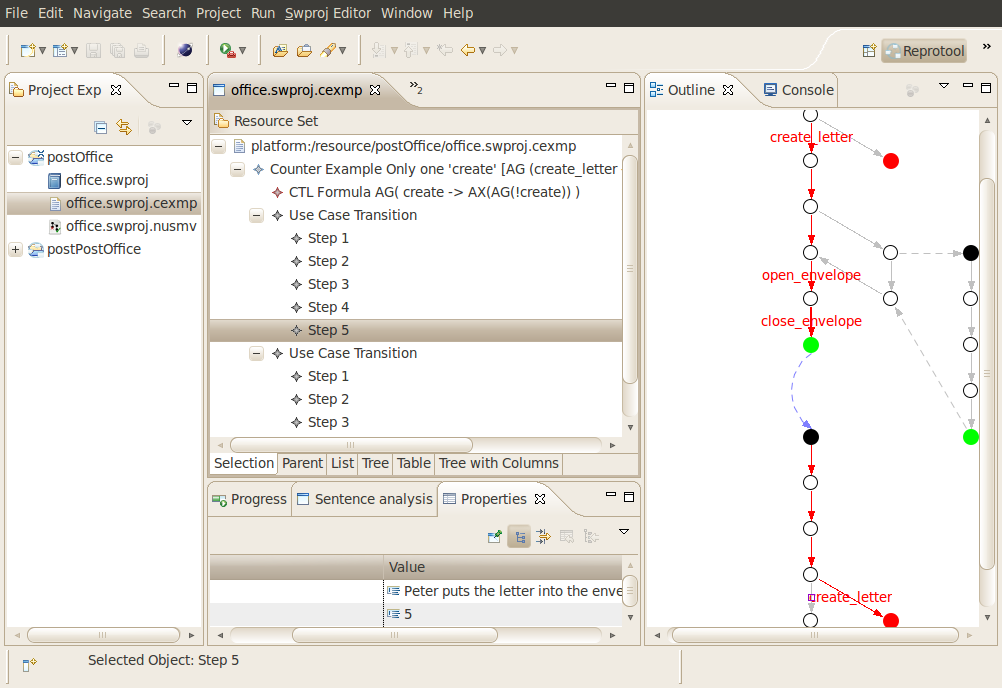
\includegraphics[height=280pt]{images/reprotoolVerify}
  \caption{Counter-example for our \emph{PostOffice} project}
  \label{fig:reprotoolVerify}
\end{figure}

This counte-example shows us the execution path that encounters the annotaion \emph{\#create\_letter} two times. And this contradicts
the default semantics of the \emph{create} annotation. According to our default semantics, the \emph{create} annotaion can be used
only once to create an object (You can not create the same object more than once). 

The easiest way how to fix our \emph{PostOffice} project is to remove one \emph{\#create\_letter} annotation. But we will take another
approach that will demonstrate the usage of the special annotations \emph{trace} and \emph{on}. We provide more information about
these \emph{special annotations} in the programmer's documentation.

Edit the \emph{writeLetter} use-case and add the \emph{\#trace\_a} annotation to the step that is right after the step annotated with
\emph{\#create\_letter}. (That means you will annotate the step thet reads \emph{Peter checks if he has a spare envelope.}) This
situation is shown in the next picture:

\begin{figure}[ht]
  \centering
  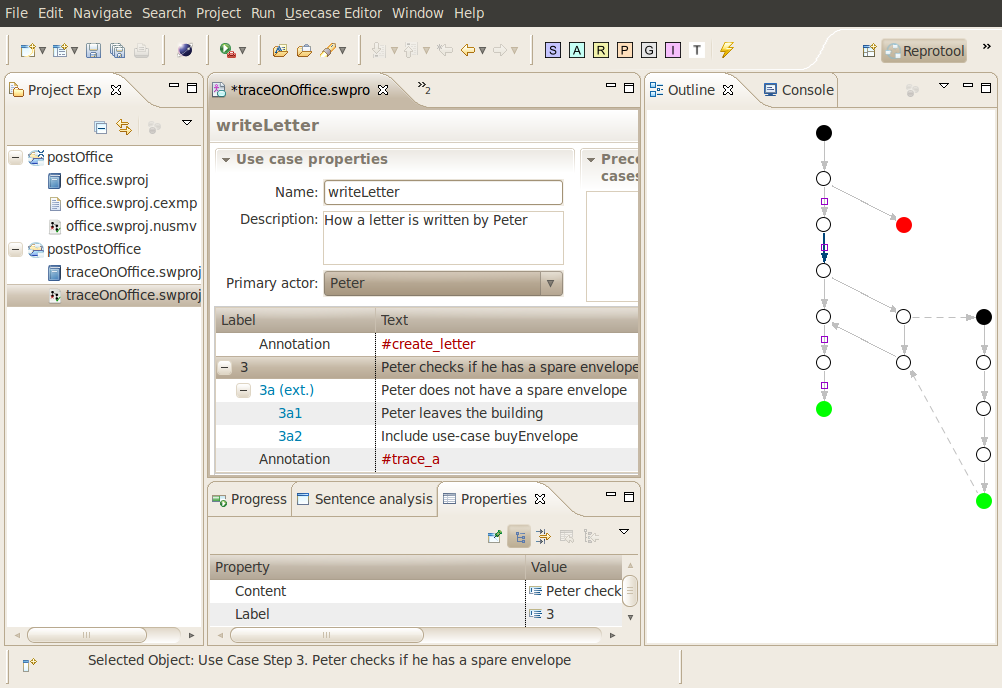
\includegraphics[height=280pt]{images/reprotoolTraceA}
  \caption{\emph{\#trace\_a} annotation added}
  \label{fig:reprotoolTraceA}
\end{figure}

\newpage

Now edit the \emph{takeLetter} use-case and add the \emph{\#on\_a} annotation to the step that already has the \emph{\#use\_letter}
annotation. (That means you will now annotate the step that reads \emph{The post officer takes the letter from Peter.}) This situation
is shown in the next picture:

\begin{figure}[ht]
  \centering
  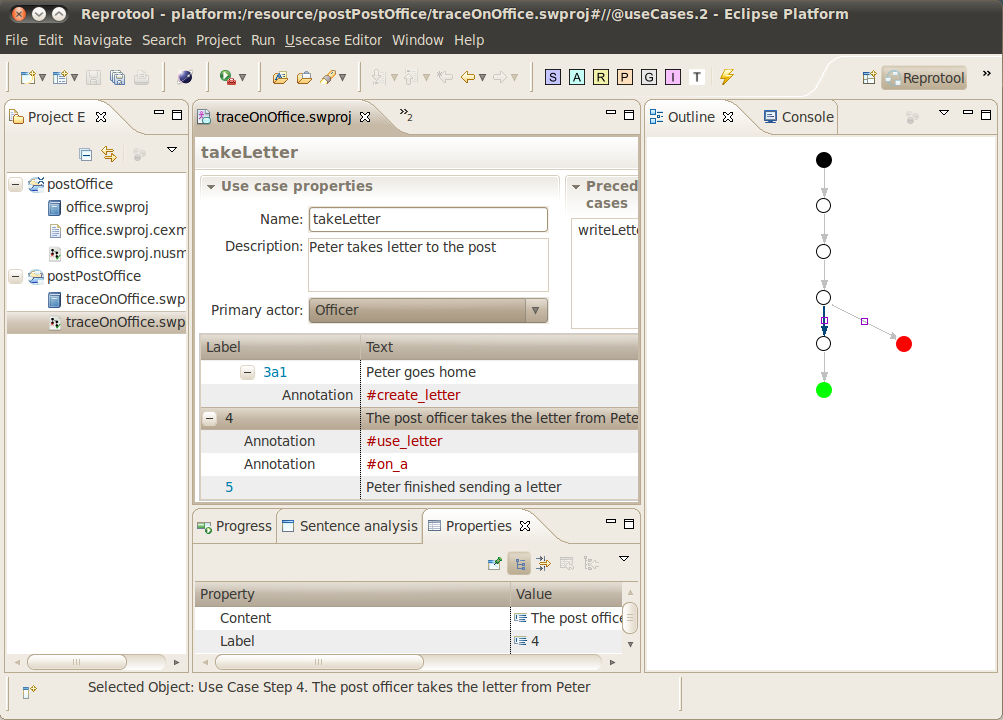
\includegraphics[height=280pt]{images/reprotoolOnA}
  \caption{\emph{\#on\_a} annotation added}
  \label{fig:reprotoolOnA}
\end{figure}

Now if you run the \emph{NuSMV} verification, the \emph{NuSMV} model checker does not consider the path in the previous counter-example
and therefore the project passes the verification process. 

\subsection{Check the example projects}
In the folder \emph{documentation} of the \emph{Reprotool} root svn directory, there is a directory \emph{exampleProjects} that you
can directly import into \emph{Reprotool}. There is the \emph{postOffice} project, the \emph{postOfficeTraceOn} project with \emph{trace}/\emph{on}
annotation pair and a couple of others that you can check. Import the projects into \emph{Reprotool} by executing this command:
\begin{verbatim}
 File / Import
\end{verbatim}
Now a dialog box appears, select \emph{General} and there click on the \emph{Existing projects into workspace}. Press Next. Now select
as the root directorythe \emph{exampleProjects} directory on your filesystem. Now click Finish - the projects should now be imported
to your \emph{eclipse workspace}.

\begin{figure}[ht]
  \centering
  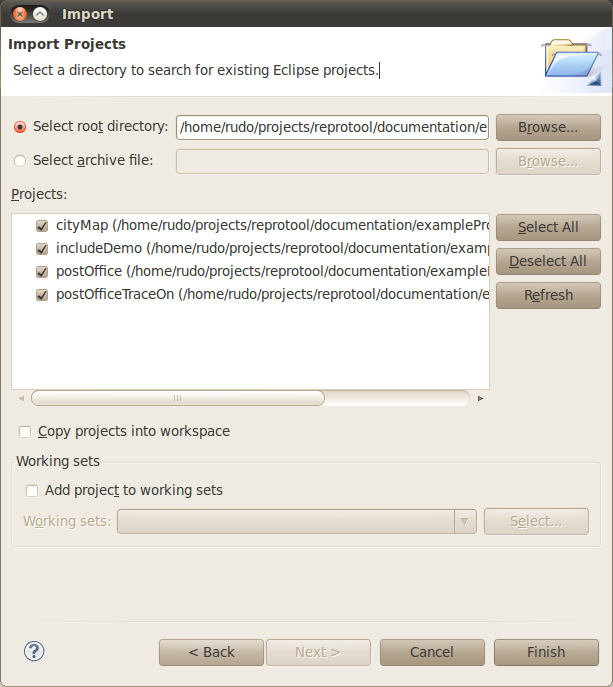
\includegraphics[width=280pt]{images/reprotoolImport}
  \caption{\emph{Reprotool} import project dialog}
  \label{fig:reprotoolImport}
\end{figure}